% Chapter 3

\chapter{Computational model} % Main chapter title
\label{chapter:computationalmodel} % For referencing the chapter elsewhere, use \ref{Chapter1} 

The previous chapter, presented the experimental model designs for the iFEM process of the material 
parameter identification, detailling the experimental setups, results, and main assumptions 
made for the material models. These foundations enabled the development of the finite element (FE) model.

In this chapter, the computational models of the indentation tests introduced in Chapter \ref{chapter:experimentalmodel} 
will be described. These models were constructed using the finite element software ANSYS. 
The computational model serves as the principal link between the experimental data and the identification of the 
specimen's material parameters.\\  

The initial simulation model, referred to as Computational model I (CP I), served as a tool 
for testing the preliminary ideas, as well as establishing the basis structure for 
the computational model. This first step was essential to identify the strengths and 
weaknesses of the model, offering insights that guided the development of an 
improved simulation model, referred to as Computational model II (CP II). By examining the 
results and challenges of computational model I, the initial conceptual ideas for FE model 
were iterated, leading to the creation of a more robust and accurate computational model
for the material parameters' identification process.

In this chapter, the development process of the computational models will discussed in detail, 
including the complications encountered, the proposed solutions, 
and the improvements made in computational model II.

%-----------------------------------------------------------------------------------------
\section{Computational model I}
\label{section:cpI}
\subsection{Middle Point}
\label{subsection:mpcpI}
The quasi-static nature of the indentation experiment for allowed the use of a static 
structural analysis. To prioritize the development of the framework for the material 
parameter identification process, the model was simplified as much as possible.
This approach minimized the influence of errors arising from complex geometries and boundary conditions.

\subsubsection*{Description}
The geometry only included key components that significantly contribute to the mechanical response,
i.e., the indenter and the specimen. The tumor extraction geometry depicted in Figure \ref{fig:specimenhole}
was also modeled for CP I. Both the indenter and the specimen utilized SOLID187 elements.
SOLID187 elements are a high order 3-D, \SI{10}{}-node elements with three degrees of freedom at each node.
These elements were suitable for simulating deformations of nearly incompressible hyperelastic materials 
and offered hyperelasticity, large deflection, and large strain capabilities \cite{Ansys2010}.\\
%Geometry model CPI
The geometry model used for EP I is shown in Figure \ref{fig:geometrycpI}. %figure of the middle point geometry for experimental model I
Although symmetry could have been applied, it was not employed in this case. This decision considered 
future projects, where the measurement and identification of human organ material parameters were desired 
objectives. For these cases, due to the material's anisotropy and the usual complex geometry,
symmetry boundary conditions could not be applied. 
\begin{figure}%
    \centering
   \quad
   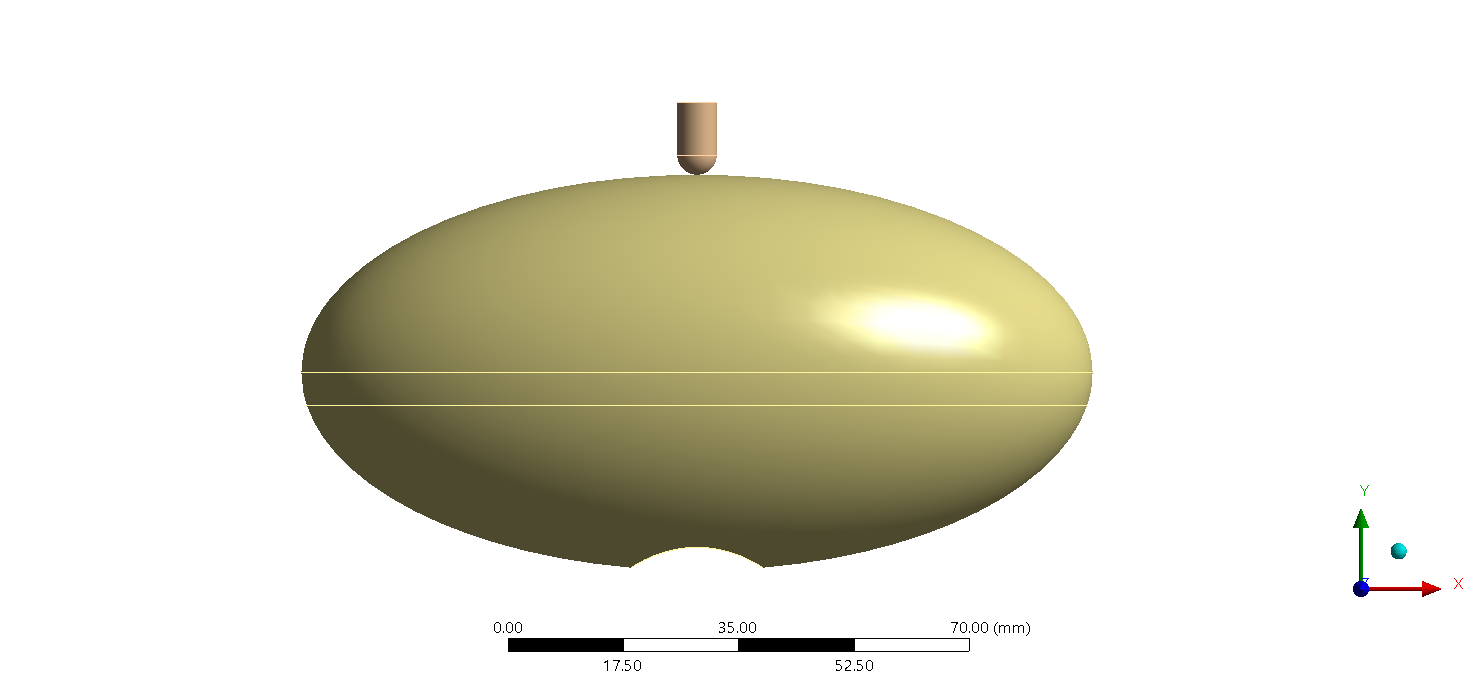
\includegraphics[width=10cm]{Images/computational/Assemblynoplatform2.png}%
   \caption[Computational model I geometry]{CP I geometry: Illustration of the geometry model with its key components, indenter and specimen with tumor extraction.}%
   \label{fig:geometrycpI}%
\end{figure}
%contact
The contact formulation between the indenter and the specimen was set to frictionless (CONTA174) to reduce
overall model complexity and mimic the lubricated contact of the experiment configuration.
The lower half of the specimen was defined as a fixed support, mirroring the physical constraint of the 
experimental setup. The displacement value $h$ was applied to the indenter in the Y-direction,
and the force reaction $F$ was subsequently obtained.\\
%Mesh
A global element size of $e_{I_s}=\SI{5}{\milli\meter}$ was applied to the specimen's mesh, which 
consisted of quadratic tetrahedral elements. The contact area between the indenter and the specimen's surface 
was refined to $e_{I_a}=\SI{0.3}{\milli\meter}$ (Fig.\ref{fig:cpImesh}). The primary reason for applying contact
sizing refinement was to ensure independence from the specimen's geometry or the indenter's position on the specimen's surface.\\
\begin{figure}
    \centering
    \begin{subfigure}[b]{0.45\textwidth}
    \centering
    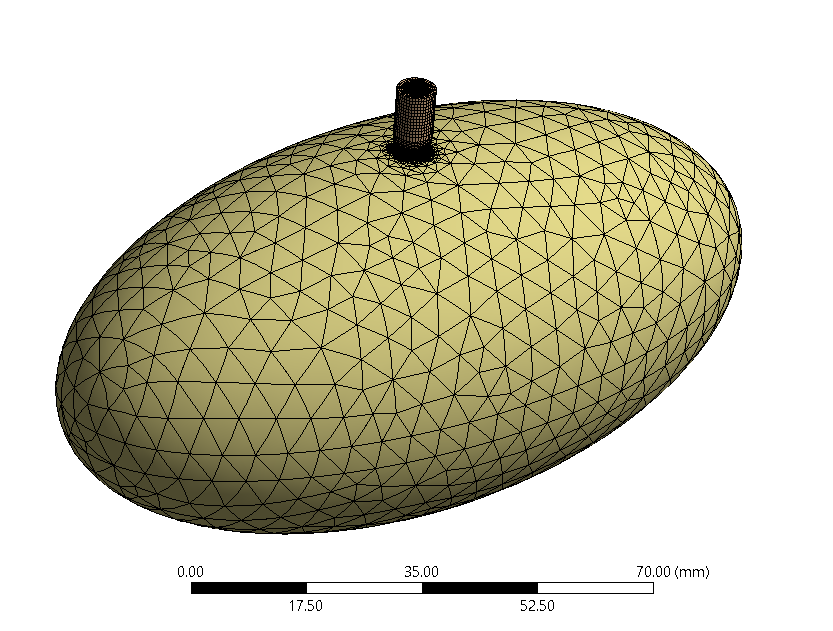
\includegraphics[width=\textwidth]{Images/computational/MeshCSES03total.png}
    \caption{Whole geometry meshing}
    \label{fig:cp1meshtotal}
    \end{subfigure}
    \hfill
    \begin{subfigure}[b]{0.45\textwidth}
    \centering
    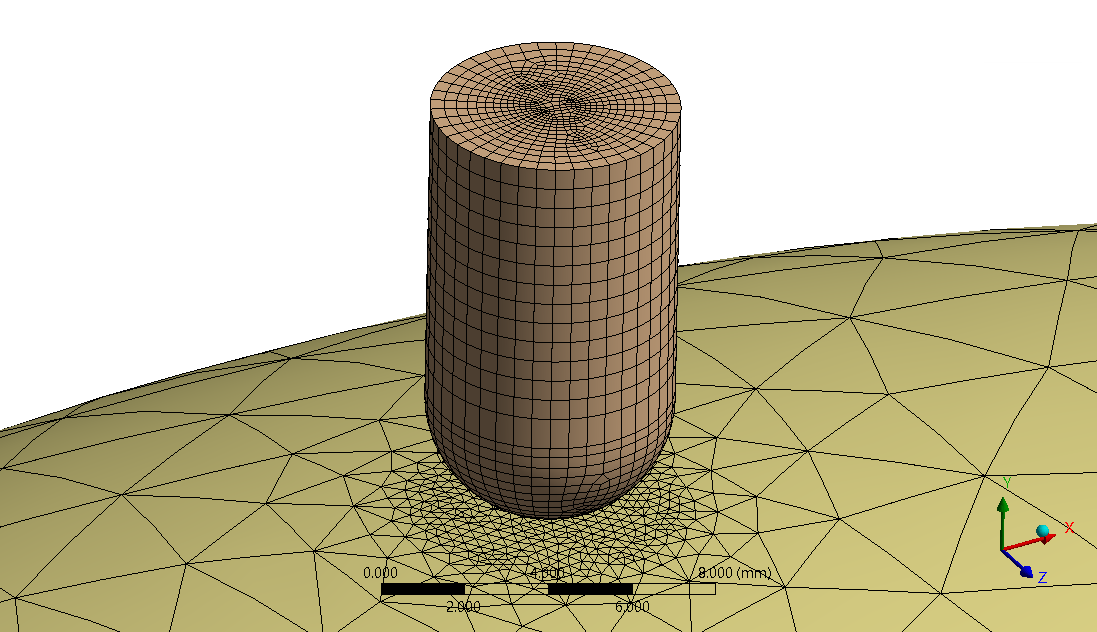
\includegraphics[width=\textwidth]{Images/computational/MeshCSES03.png}
    \caption{Mesh refinement area}
    \label{fig:cp1meshref}
    \end{subfigure}
    \hspace{0.3cm}
    \caption[Computational model I mesh]{CP I mesh: Patch conforming mesh with contact sizing refinement in the contact between the indenter and the specimen's surface.}
    \label{fig:cpImesh}
\end{figure}
Finally, initial parameters were assigned to the computational model to approximate the mechanical properties of ultra-soft polyurethane. 
For the linear elasticity level, values for the Young's modulus $E$ and the Poisson's ratio $\nu$ were assigned. 
From the main assumptions made in Section \ref{section:mainassumption},the Poisson's ratio for the first 
level material model was set to $\nu =  0.49$, and the Young's modulus was calculated using equation \ref{eq:forcelinear}
\begin{align}
    E = \frac{3F(1-\nu^2)} {4{r_i}^{\frac{1}{2}} {h}^{\frac{3}{2}}}\, .
    \label{eq:forcelinearcp1}
\end{align}
Substituting the indenter radius $r_i =  \SI{3}{\milli \meter}$ and the indentation depth $h =  \SI{3.8}{\milli \meter}$ a Young's modulus $E_{LE}$ was calculated and resulted in 
\begin{align}
    E_{LE} = 0.018 MPa \approx 0.02 MPa \, .
    \label{eq:Elinearcp1}
\end{align}


\subsubsection*{Level 1 Results}
An indentation depth of $h = \SI{3.8}{\milli \meter}$ could not be solved with the linear elastic material model. 
Through an iterative process, it was discovered that the linear elastic material model could only be applied 
up to an indentation depth of $h \approx \SI{2}{\milli \meter}$.\\

The initial attempt to match the experimental and simulation data provided a reasonable approximation of the experimental data.
Figure \ref{fig:MPI2mmvsCPILE} demonstrates the comparison between the experimental data and the CP I using a 
linear elastic material model up to an indentation depth of $h = \SI{2}{\milli \meter}$. The CP I curve displayed 
a more pronounced curvature than the experimental data. Additionally, at $u =\SI{0}{\milli \meter}$, 
this curve exhibited a steeper initial slope; however, as the displacement increased, the 
difference in slope between the two curves diminished.\\

This result indicated that for a displacement greater than $h = \SI{2}{\milli \meter}$, the CP I curve would 
lie above the experimental data. Interestingly, it was observed that, despite employing a linear elastic model, 
the force-displacement curve exhibited a nonlinear response. This observation suggested that even a relatively 
simple material model could capture some degree of nonlinearity. 

\begin{figure}%
    \centering
   \quad
    \begin{tikzpicture}[scale=1]
        \begin{axis}[
            xmax=2.2,xmin=0,
            ymin= 0,ymax=0.2,
            %ytick={0,0.1,0.2,...,0.6},
            xlabel={Displacement $u [mm]$},
            ylabel={Force reaction $F_{MP} [N]$},
            grid = major,
            legend pos= north west]
            \addplot+[smooth, no markers, thick] table [y=$Force$, x=Def]{Table/CP1/MPI2mm.dat};
            \addplot+[smooth, no markers, thick] table [y=$Force$, x=Def]{Table/CP1/CP12mmCSfullmodelLE.dat};
            \legend{Experiment I,CP I-LE}
        \end{axis}
    \end{tikzpicture}%
   \caption[Computational model I vs Experimental data - Linear elasticity]{CP I vs EP I: Comparison of force-displacement curves between experimental data for Middle Point case and the initial computational model with a linear elastic model for $h = \SI{2}{\milli \meter}$.}%
   \label{fig:MPI2mmvsCPILE}%
\end{figure}


\subsubsection*{Level 2 Results}
At the hyperelastic level, the initial parameters for the Neo-Hookean model, 
the shear modulus $\mu$ and the incompressibility parameter $D_1$ were calculated from the Young's modulus $E_{LE}$
and the Poisson's ratio $\nu$ from the linear elastic model. With equation \ref{eq:mucp1}, \ref{eq:bulkmodcp1}, 
and \ref{eq:incomparcp1}, the shear modulus $\mu_{CPI}$ and the incompressibility parameter $D_{1_{CPI}}$
\begin{align}
    \mu_{CPI} = 0.0067 MPa \, ,
    \label{eq:mucp1result}
\end{align}
\begin{align}
    D_{1_{CPI}} = 6 MPa \, ,
    \label{eq:d1cp1result}
\end{align}
were calculated, respectively. These parameters were integrated in the model described above. In comparison from 
the linear elastic model, the Neo-Hookean material model could solve the simulation for an indentantion depth of 
$h =  \SI{3.8}{\milli \meter}$.
\begin{figure}%
    \centering
   \quad
    \begin{tikzpicture}[scale=1]
        \begin{axis}[
            xmax=4.2,xmin=0,
            ymin= 0,ymax=0.6,
            ytick={0,0.1,0.2,...,0.5},
            xlabel={Displacement $u [mm]$},
            ylabel={Force reaction $F_I [N]$},
            grid = major,
            legend pos= north west]
            \addplot+[smooth, no markers, thick] table [y=$Force$, x=Def]{Table/Middle Point/MPI38mm.dat};
            \addplot+[smooth, no markers, thick] table [y=$Force$, x=Def]{Table/CP1/CP1CSfullmodelNH.dat};
            \legend{Experiment I,CP I-NH}
        \end{axis}
    \end{tikzpicture}%
   \caption[Computational model I vs Experimental data - Neo-Hookean]{CP I vs EP I: Comparison of force-displacement curves between experimental data for Middle Point case and the initial computational model with a Neo-Hookean model for $h = \SI{3.8}{\milli \meter}$.}%
   \label{fig:MPIvsCPINH}%
\end{figure}
The Neo-Hookean simulation curve displayed a slightly steeper slope at lower values of $u$ in comparison to the experimental data.
As the displacement $u$ increased, the difference in slope between the two curves decreased, inidicating that the 
curves approached certain parallelism around $u = \SI{3.8}{\milli \meter}$.\\

Despite the discrepancies between the two curves, the Neo-Hookean provided a fair approximation to the experimental data, considered the 
given displacement range. Likewise, this outcome evidenced that the Neo-Hookean model was capable of capturing some of the nonlinear 
response observed in the experimental data, by directly inputing the calculated values from the linear elastic material model.
Nevertheless, it is important to note that improvements to the computational model are necessary to achieve a more
accurate representation of the experimental results.

\section{Analysis and Complications}
\label{section:challengescp}
\subsection{Verification of the Computational Model}
The verification of the computational model was an important aspect of ensuring the accuracy and reliability of the 
the simulation results. One typical approach to verify the model is to conduct a mesh convergence analysis. To 
reduce computational time, symmetry boundary conditions were applied, and one-quarter of CP I was used.

\subsubsection*{Mesh Convergence Analysis}
The FE model utilized for the mesh convergence analysis possessed a global element size of $e_{I_s}=\SI{5}{\milli\meter}$ 
and $e_{I_i}=\SI{1}{\milli\meter}$. The previous results showed that only the area of interest was relevant for the 
calculations and a refinement was made for this area. The contact are between the indenter and the specimen's surface



A typical approach to verify the computational model is to conduct a mesh convergence analysis.
To reduce computational time the symmetry boundary conditions were used, therefore one-quarter model was used for EP I.  
The convergence FE model possessed an global element size of $e_{I_s}=\SI{5}{\milli\meter}$ and $e_{I_i}=\SI{1}{\milli\meter}$ for the specimen 
and the indenter respectively. A refinement was made in the area of interest, i.e., the contact 
area between the indenter and the specimen's surface, with a sphere radius of 
$r_{I_a}=\SI{8}{\milli\meter}$ and an element size of $e_{I_a}=\SI{0.5}{\milli\meter}$.

The mesh convergence supposed a challenge because the smaller the element from 5mm to 0.1 mm in the contact area,
some of the results could not solve due to large element deformation problems or there was some values, which were 
very deviated from the tendency curve. Nevertheless, a certain tendency to convergence was observed.





\subsubsection*{Stress Distribution Analysis}
%best result with convergence
The mesh for the whole model were formed from quadratic tetrahedral elements. 
Various meshing methods were tried and the mesh, which showed the best results for experimental model I 
possessed an global element size of $e_{I_s}=\SI{5}{\milli\meter}$ and $e_{I_i}=\SI{1}{\milli\meter}$ for the specimen 
and the indenter respectively. A refinement was made in the area of interest, i.e., the contact 
area between the indenter and the specimen's surface, with a sphere radius of 
$r_{I_a}=\SI{8}{\milli\meter}$ and an element size of $e_{I_a}=\SI{0.5}{\milli\meter}$ (Fig.). %add meshing figure.
Their a two main factors which increases the complexity of the validation of the simulation
and those are, the contact nonlinearity, and the element distortion due to indentation
 experiment. These issues make the computational time expensive, as it requires to manual 
 solutions for the meshing in the area of importance, and small time steps. 
 For that, 
 the nonlinear adaptive meshing option in ANSYS Workbench was applied, which does a remeshing
 process if the a certain parameter is exceeded.%Revisar explanation of nonlinear adaprive meshing
Specially, for larger indentation cases, this option shows a more stable model with a 
good mesh convergence analysis.

A force-displacement curve, shown in Fig... is generated from the first assumption, 
for this case 
%Additionally due to these factors, the converge analysis   

\section*{Experimental model II}
This was removed for the EP II geometry model, as it was shown that this area 
of the specimen's geometry was irrelevant for the calculation of the results.
For EP I and EP II only one-quarter, and the half of the full model was used respectively.
The decision to use half model for EP II was made to make the visualization of the deformation profile 
easier for the validation in further steps.\\

The mesh for the whole model is formed from quad tetrahedral elemennts. The platform and 
the specimen have an global element size of 5 mm. The indenter has an element size of
0.5 mm. In the area of the indentation, there is finer mesh with an element size of
1 mm and a radius of 8 mm. 



For both cases 

\subsection{Verification of the Simulation Model}

\subsubsection*{Mesh Convergence Analysis}
\subsubsection*{Platform vs Fixed Support}


%----------------------------------------------------------------------------------
\section{Nearby point}


